%\newcommand{\emptysmodel}[0]{$\textbf{\LARGE{X}}$}
%\usetikzlibrary {positioning}
\newcommand{\setsets}[1]{\boldsymbol{#1}}
\newcommand{\App}[1]{\ensuremath{A_{#1}}}
\newcommand{\A}[2]{\App{#1}#2}
\newcommand{\Appfixp}[1]{\ensuremath{A_{#1}^{*}}}
\newcommand{\Afixp}[2]{\Appfixp{#1}#2}
\newcommand{\Appi}[2]{\ensuremath{A_{#1}^{#2}}}
\newcommand{\Ai}[3]{\Appi{#1}{#2}#3}

\tikzset{% 
    examples/.style={%
->
, x=1.5cm
, y=-1.5cm
, smodel/.style={rectangle,minimum size=0.5cm,draw,thin, rounded corners}
%, empty/.style={minimum size=7mm}
, arrow/.style={<-,thin}
%, empty_arrow/.style={arrow,dotted,draw=none} % dashed
, rule/.style={align=center, draw}
, rule_arrow/.style={<-}
, clingo/.style={font=\small\ttfamily,draw,align=left}
, clingo_rule/.style={font=\small\ttfamily,align=left}
    }
}

% ----------------------------------------------------------------------
\begin{frame}{Example}

$
P
=
\left\{
    \only<1>{\{ p \} \leftarrow,}\only<2->{q \leftarrow p,} \
    \only<1>{q \leftarrow p,}\only<2>{\{ p \} \leftarrow,}\only<3->{\phantom{q} \leftarrow \naf{q},} \
    \only<1-2>{\phantom{q} \leftarrow \naf{q}}\only<3->{\{ p \} \leftarrow} 
\right\}
$

\begin{center}
\begin{tikzpicture}
[examples
]

%\draw [help lines] (0,0) grid (-5,5);

% line 0

\node[smodel] (node01)  at ( 1, 0) {};

% line 1

\node[smodel] (node11) at ( 0,1) {}
  edge [arrow] (node01);

\node[smodel] (node12) at ( 2,1) {$p$}
  edge [arrow] (node01);

\only<1-3>{
\node[rule] (rule1) at (3.5,1) {$\{p\} \leftarrow$};
}
\visible<4>{
\draw (2.75,0.75) node[anchor=south west,align=right] {\texttt{example.lp}} rectangle (4.25,3.25) ;

\node[clingo_rule] at (3.5,1) {\{p\}.};
}

% line 2

\node[smodel] (node21) at ( 0,2) {}
  edge [arrow] (node11);

\node[smodel] (node22) at ( 2,2) {$p$ $q$}
  edge [arrow] (node12);

\only<1-3>{
\node[rule] (rule2) at (3.5,2) {$q \leftarrow p$}
  edge [rule_arrow] (rule1);
}
\only<4>{
\node[clingo_rule] at (3.5,2) {q :- p.};
}

% line 3

%\node[empty] (node31) at ( 0,3) {\emptysmodel}
%  edge [empty_arrow] (node21);

\node[smodel] (node32) at ( 2,3) {$p$ $q$}
  edge [arrow] (node22);

\only<1-3>{
\node[rule] (rule3) at (3.5,3) {$\phantom{q} \leftarrow \naf{q}$}
  edge [rule_arrow] (rule2);
}
\only<4>{
\node[clingo_rule] at (3.5,3) {:- not q.};
}

\end{tikzpicture}
\end{center}

\end{frame}


% ----------------------------------------------------------------------
\begin{frame}{Example}

$
P
=
\left\{
    \{ p \} \leftarrow, \ \
    q \leftarrow p, \ \
    \{ r \} \leftarrow \naf{p}, \ \
    s \leftarrow \naf{r}, \naf{q}, \ \
    \phantom{s} \leftarrow r, p
\right\}
$

\begin{center}
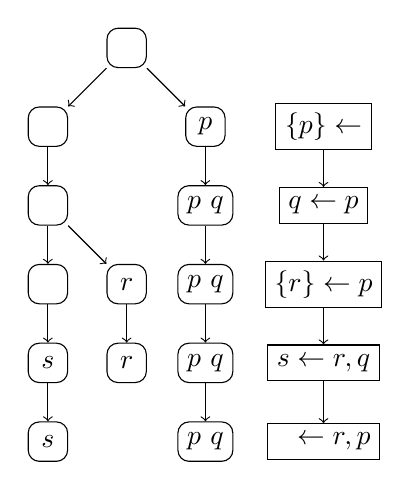
\begin{tikzpicture}
[examples
, x=1cm
, y=-1cm
]

%\draw [help lines] (0,0) grid (-5,5);

% line 0

\node[smodel] (node01)  at ( 1, 0) {};

% line 1

\node[smodel] (node11) at ( 0,1) {}
  edge [arrow] (node01);

\node[smodel] (node12) at ( 2,1) {$p$}
  edge [arrow] (node01);

%\only<1-3>{
\node[rule] (rule1) at (3.5,1) {$\{p\} \leftarrow$};
%}
%\visible<4>{
%\draw (2.75,0.75) node[anchor=south west,align=right] {\texttt{example.lp}} rectangle (4.25,3.25) ;
%
%\node[clingo_rule] at (3.5,1) {\{p\}.};
%}

% line 2

\node[smodel] (node21) at ( 0,2) {}
  edge [arrow] (node11);

\node[smodel] (node22) at ( 2,2) {$p$ $q$}
  edge [arrow] (node12);

%\only<1-3>{
\node[rule] (rule2) at (3.5,2) {$q \leftarrow p$}
  edge [rule_arrow] (rule1);
%}
%\only<4>{
%\node[clingo_rule] at (3.5,2) {q :- p.};
%}

% line 3

\node[smodel] (node31) at ( 0,3) {}
  edge [arrow] (node21);

\node[smodel] (node32) at ( 1,3) {$r$}
  edge [arrow] (node21);

\node[smodel] (node33) at ( 2,3) {$p$ $q$}
  edge [arrow] (node22);

%\only<1-3>{
\node[rule] (rule3) at (3.5,3) {$\{r\} \leftarrow \naf{p}$}
  edge [rule_arrow] (rule2);
%}
%\only<4>{
%\node[clingo_rule] at (3.5,3) {r :- not q.};
%}

% line 4

\node[smodel] (node41) at ( 0,4) {$s$}
  edge [arrow] (node31);

\node[smodel] (node42) at ( 1,4) {$r$}
  edge [arrow] (node32);

\node[smodel] (node43) at ( 2,4) {$p$ $q$}
  edge [arrow] (node33);

%\only<1-3>{
\node[rule] (rule4) at (3.5,4) {$s \leftarrow \naf{r}, \naf{q}$}
  edge [rule_arrow] (rule3);

% line 5

\node[smodel] (node51) at ( 0,5) {$s$}
  edge [arrow] (node41);

%\node[smodel] (node42) at ( 1,4) {$r$}
%  edge [arrow] (node32);

\node[smodel] (node53) at ( 2,5) {$p$ $q$}
  edge [arrow] (node43);

%\only<1-3>{
\node[rule] (rule5) at (3.5,5) {$\phantom{s} \leftarrow r, \naf{p}$}
  edge [rule_arrow] (rule4);

\end{tikzpicture}
\end{center}

\end{frame}

\begin{frame}{\only<1>{Normal logic programs}\only<2->{Extended logic programs}}
  \label{eqn:rule}
  \begin{itemize}
  \item %<1->
    A \alert<1>{logic program}, $P$, over a set $\mathcal{A}$ of atoms is a finite \alert<1>{set} of rules
  \item %<1->
    A \only<1>{(normal)}\alert<2-4>{\only<2>{normal}\only<3>{choice}\only<4>{constraint}} \alert{rule}, $r$, is of the form
    \[
%      \alt<2>{\tt a_0\texttt{ :- } a_1,\dots,a_m,\texttt{ not }{a_{m+1}},\dots,\texttt{ not }{a_n}.}%
                  {\only<1-2>{a_0}\only<3>{\{a_0\}}\only<4>{\phantom{\{a_0\}}} \leftarrow   a_1,\dots,a_m,          \naf{a_{m+1}},\dots,          \naf{a_n}}
    \]
    where $0\leq m\leq n$ and each $a_i\in{\mathcal{A}}$ is an atom for $\alt<4>{1}{0}\leq i\leq n$
  \item %<3->
    \structure{Notation}
    \begin{align*}
      \head{r}\phantom{^+}    &=\, \only<1-3>{a_0}\only<4>{\{\}}
      \\
      \body{r}\phantom{^+}    &=\, \{a_1,\dots,a_m,\naf{a_{m+1}},\dots,\naf{a_n}\}
      \\
      \pbody{r}               &=\, \{a_1,\dots,a_m\}
      \\
      \nbody{r}               &=\, \{a_{m+1},\dots,a_n\}
%     \only<4>{%
%      \\
%      \atom{P}\phantom{^+} &=\, \textstyle\bigcup_{r\in P}\left(\{\head{r}\}\cup\pbody{r}\cup\nbody{r}\right)
%      \\
%      \body{P}\phantom{^+} &=\, \{\body{r}\mid r\in P\}
%      \\
%      \head{P}\phantom{^+} & =\, \{\head{r}\mid r\in P\}}
    \end{align*}%
  \item %<4-> 
  A \alert<1>{literal} is an atom or a negated atom
  \item %<5-> 
  A program $P$ is \alert<1>{positive} if $\nbody{r}=\emptyset$ for all $r\in P$
  \end{itemize}
\end{frame}


%\renewcommand{\head}[1]{\ensuremath{\mathit{h}(#1)}}
%\renewcommand{\body}[1]{\ensuremath{\mathit{b}(#1)}}

\newcommand{\headphantom}[1]{\ensuremath{\phantom{\mathit{head}(}#1\phantom{)}}}

% ----------------------------------------------------------------------
\begin{frame}<1-4>[label=operatorframe]{Application operator}
  \begin{itemize}
  \item A set of atoms $X$ \alert<1>{satisfies} a set of literals \mbox{\small$\{a_1,\dots,a_m,\naf{a_{m+1}},\dots,\naf{a_n}\}$} if
      \mbox{\small$\{a_1, \dots, a_m\} \subseteq X$} and \mbox{\small$\{a_{m+1},\dots,a_n\} \cap X = \emptyset$}.
\medskip
  \item<2-> Let $P$ be a set of \alert<2-5>{\only<2>{normal}\only<3>{choice}\only<4-5>{constraint}} rules and $\setsets{X}$ a set of sets of atoms,

 \par     the \alert<2>{application operator} $\App{P}$ is defined as follows:
      \smallskip 

\mbox{\small$
      \A{P}{\setsets{X}} = \big\{  
        \only<1-3>{X \cup Y}\only<4-5>{\alert<4-5>{\hspace{9.5pt}X \hspace{10pt}}}\mid X \in \setsets{X}, \only<1-3>{Y}\only<4-5>{\ \alert<4-5>{\emptyset}} \only<1-2,4-5>{=}\only<3>{\alert<3>{\subseteq}} \{ \only<1-3>{\head{r}}\only<4-5>{\hspace{14.5pt} \alert<4-5>{r} \hspace{14pt}} \mid r\in P\text{ and } M \text{ satisfies } \body{r} \} %\pbody{r}\subseteq X\text{ and } \nbody{r}\cap X=\{\} \}
      \big\}
      $}
      \smallskip 

%  \item \structure{Example:}
\visible<5>{
   \item For $n \geq 1$, let $\Ai{P}{n}{\setsets{X}}$ be $\A{P}{\setsets{X}}$ if $n=1$ and $\Ai{P}{n-1}{\A{P}{\setsets{X}}}$ if $n > 1$.
   \item Let $\Afixp{P}{\setsets{X}}$ be $\Ai{P}{n}{\setsets{X}}$ where $n$ is the smallest integer such that 
        $\Ai{P}{n}{\setsets{X}}=\Ai{P}{n+1}{\setsets{X}}$ 
}
  \end{itemize}

\end{frame}

% ----------------------------------------------------------------------
\begin{frame}{Non-recursive programs}
  \begin{itemize}
    \item Dependency graph of program $P$
      \begin{itemize}
        \item rule $r_2$ depends on rule $r_1$
              if $(\pbody{r_2}\cup\nbody{r_2})\cap\head{r_1}\neq\emptyset$
        \item $G_P=(P,E)$ where $E=\{ (r_1,r_2) \mid r_2 \mbox{ depends on } r_1 \}$
      \end{itemize}
    \item Program $P$ is non-recursive if $G_P$ is acyclic, i.e., it has no path of length greater than zero
          from some rule $r$ to itself
    \item If $P$ is non-recursive then there is some topological ordering
          $(r_1, \ldots, r_n)$
          of $G_P$, and
          for all such orderings the results of
          $\A{\{r_n\}}{\ldots\A{\{r_1\}}{\{\emptyset\}}}$
          coincide and are equal to the stable models of $P$
  \end{itemize}
\end{frame}

% ----------------------------------------------------------------------
\begin{frame}{Non-recursive programs}
  \begin{itemize}
    \item If $P$ is non-recursive then there is
          some ordering $(p_1, p_2, \ldots)$ of the atoms of $P$ along with
          some topological ordering
          $(r_1, \ldots, r_n)$ of $G_P$ where:
    \begin{itemize}
      \item first occur the facts, 
      \item then the normal rules whose head is $p_1$, 
      \item then the choice rules whose head is $p_1$, 
      \item then the constraint rules that are independent of the rest of the rules,
      \item then the normal rules whose head is $p_2$, 
      \item then the choice rules whose head is $p_2$, 
      \item and so on\ldots
    \end{itemize}
    %for some ordering $(p_1, p_2, \ldots)$ of the atoms of $P$ 
    \item $\A{C_n}{\ldots\A{C_m}{\A{C_{m+1}}{\ldots\A{C_1}{\{\emptyset\}}}}} =
           \A{C_n}{\ldots\A{C_m \cup C_{m+1}}{\ldots\A{C_1}{\{\emptyset\}}}}$ whenever 
            the rules of $C_m$ do not depend on the rules of $C_{m+1}$ and vice versa
    \item Then we can group in separate components
          the normal, choice and constraint rules for every atom, and also the initial facts
  \end{itemize}

%\begin{textblock*}{\textwidth}(.75\textwidth,0.25\textheight)
%    \begin{beamercolorbox}[wd=.5\textwidth,center,sep=0.3cm]{block body example}
%        This is wrong!
%    \end{beamercolorbox}
%\end{textblock*}

%\begin{tikzpicture}[remember picture,overlay]
%\node at (current page.center) {\alert{ground}};
%\node at (3,0.5) {\alert{\Huge{ground}}};
%\draw[step=1,help lines] (0,0) grid (10,10);
%\end{tikzpicture}

\end{frame}

% ----------------------------------------------------------------------
\againframe<5>{operatorframe}

% ----------------------------------------------------------------------
\begin{frame}{Easy programs}
  \begin{itemize}
    \item Dependency graph of program $P$
      \begin{itemize}
        \item rule $r_2$ depends on rule $r_1$
              if $(\pbody{r_2}\cup\nbody{r_2})\cap\head{r_1}\neq\emptyset$
        \item $G_P=(P,E)$ where $E=\{ (r_1,r_2) \mid r_2 \mbox{ depends on } r_1 \}$
        \item an edge $(r_1,r_2)$ is negative if $\nbody{r_2}\cap\head{r_1}\neq\emptyset$
      \end{itemize}
    \item Program $P$ is easy if in $G_P$ every path from some rule $r$ to itself
     \begin{itemize}
       \item does not contain negative edges, and 
       \item does not include rules of different types
     \end{itemize} 
    \item If $P$ is easy then there is some topological ordering
          $(C_1, \ldots, C_n)$ of the strongly connected components
          of $G_P$ such that the components $C_i$ do not contain rules of different types, and
          for all such orderings the results of
          $\Afixp{C_n}{\ldots\Afixp{C_1}{\{\emptyset\}}}$
          coincide and are equal to the stable models of $P$
    \item Note: 
          The $C_i$'s are either sets of recursive rules, or
          singleton sets $\{r\}$ where $r$ is not recursive,
          in which case $\Appfixp{{\{r\}}}=\App{\{r\}}$.
  \end{itemize}
\end{frame}

% ----------------------------------------------------------------------
\begin{frame}{Easy programs}
  \begin{itemize}
    \item If $P$ is easy then there is 
          some ordering $(X_1, \ldots, X_n)$ of a partition of the atoms of $P$ along with
          some topological ordering
          $(C_1, \ldots, C_n)$ of the strongly connected components of $G_P$
          where:
    \begin{itemize}
      \item first occur the facts, 
      \item then the non-recursive normal rules whose head is in $X_1$, 
      \item then the non-recursive choice rules whose head is in $X_1$, 
      \item then the recursive rules whose head is in $X_1$, 
      \item then the constraint rules that are independent of the rest of the rules,
      \item then the non-recursive normal rules whose head is in $X_2$, 
      \item and so on\ldots
    \end{itemize}
    %for some ordering $(p_1, p_2, \ldots)$ of the atoms of $P$ 
      \item $\Afixp{C_n}{\ldots\Afixp{C_m}{\Afixp{C_{m+1}}{\ldots\Afixp{C_1}{\{\emptyset\}}}}} =
             \Afixp{C_n}{\ldots\Afixp{C_m \cup C_{m+1}}{\ldots\Afixp{C_1}{\{\emptyset\}}}}$ whenever 
            the rules of $C_m$ do not depend on the rules of $C_{m+1}$ and vice versa
    \item Then we can group in separate components
          the normal, choice, recursive  and constraint rules for every partition, and also the initial facts
  \end{itemize}
\end{frame}

% ----------------------------------------------------------------------
\begin{frame}{Dependencies}
  \begin{tikzpicture}[
%      ->,
      y=-8mm,
      node distance=5mm,
%      every node/.style={font=\small\ttfamily},
%      node/.style={circle,minimum size=5mm,draw},
%      start/.style={circle,double=bg,minimum size=5mm,draw}]
]
    \node (omit) at (0,0) [draw,anchor=west] {omit(X,Y) :- not {{path(X,Y)}}, edge(X,Y).};
    \node [left=of omit] { Component\(_{1,1}\): };

%%%    \node (path) at (0,1) [draw,anchor=west] {path(X,Y) :- not omit(X,Y), edge(X,Y).};
%%%    \node [left=of path] { Component\(_{1,2}\): };
%%%    \node (inde) at (0,2) [draw,anchor=west] {:- path(X,Y), path(X',Y), X < X'.};
%%%    \node [left=of inde] { Component\(_{2,1}\): };
%%%    \node (outd) at (0,3) [draw,anchor=west] {:- path(X,Y), path(X,Y'), Y < Y'.};
%%%    \node [left=of outd] { Component\(_{3,1}\): };
%%%    \node (onpa) at (0,4) [draw,anchor=west] {on\_path(Y) :- path(X,Y), path(Y,Z).};
%%%    \node [left=of onpa] { Component\(_{4,1}\): };
%%%    \node (conp) at (0,5) [draw,anchor=west] {:- node(X), not on\_path(X).};
%%%    \node [left=of conp] { Component\(_{5,1}\): };
%%%    \node (star) at (0,6) [draw,anchor=west] {reach(X) :- start(X).};
%%%    \node [left=of star] { Component\(_{6,1}\): };
%%%    \node (reac) at (0,7) [draw,anchor=west] {reach(Y) :- {{reach(X)}}, path(X,Y).};
%%%    \node [left=of reac] { Component\(_{7,1}\): };
%%%    \node (crea) at (0,8) [draw,anchor=west] {:- node(X), not reach(X).};
%%%    \node [left=of crea] { Component\(_{8,1}\): };

%%%    \coordinate (lomi) at ($(omit.west)-(3mm,0mm)$);
%%%    \coordinate (romi) at ($(omit.east)+(3mm,0mm)$);
%%%    \coordinate (upat) at ($(path.west)-(3mm,-1mm)$);
%%%    \coordinate (dpat) at ($(path.west)-(3mm,+1mm)$);
%%%    \coordinate (dsta) at ($(star.east)+(3mm,-1mm)$);
%%%    \coordinate (usta) at ($(star.east)+(3mm,+1mm)$);
%%%    \coordinate (rrea) at ($(reac.east)+(3mm,0)$);
%%%    \coordinate (ronp) at ($(onpa.east)+(3mm,0)$);
%%%    \coordinate (rdst) at ($(dsta)+(3mm,0)$);
%%%    \draw [dashed] (omit) -- (lomi) -- (upat) -- (upat-|path.west);
%%%    \draw [dashed] (path) -- (romi|-path) -- (romi) -- (omit);
%%%    \draw (dpat -| path.west) -- (dpat) -- (dpat |- reac) -- (reac);
%%%    \draw (dpat |- inde) -- (inde);
%%%    \draw (dpat |- outd) -- (outd);
%%%    \draw (dpat |- onpa) -- (onpa);
%%%    \draw (star.east |- dsta) -- (dsta) -- (dsta |- reac.north);
%%%    \draw [dashed] (star.east |- usta) -- (usta -| rrea) -- (rrea |- crea) -- (crea);
%%%    \draw [-,dashed] (rrea) -- (reac);
%%%    \draw [dashed] (onpa) -- (ronp) -- (ronp|-conp) -- (conp);
%%%    \draw [-] (reac.north-|rdst) -- (rdst) -- (dsta);
%%%    \fill (dpat |- inde) circle [radius=1pt]
%%%          (dpat |- outd) circle [radius=1pt]
%%%          (dpat |- onpa) circle [radius=1pt]
%%%          (dsta) circle [radius=1pt]
%%%          (rrea) circle [radius=1pt];
  \end{tikzpicture}
\end{frame}

\begin{frame}{Normal logic programs}
  \label{eqn:rule}
  \begin{itemize}
  \item <1->
    A \alert{logic program}, $P$, over a set $\mathcal{A}$ of atoms is a finite \alert{set} of rules
  \item <1->
    A (normal) \alert{rule}, $r$, is of the form
    \[
      \alt<2>{\tt a_0\texttt{ :- } a_1,\dots,a_m,\texttt{ not }{a_{m+1}},\dots,\texttt{ not }{a_n}.}%
                  {a_0 \leftarrow   a_1,\dots,a_m,          \naf{a_{m+1}},\dots,          \naf{a_n}}
    \]
    where $0\leq m\leq n$ and each $a_i\in{\mathcal{A}}$ is an atom for $0\leq i\leq n$
    \pause
  \item <3->
    \structure{Notation}
    \begin{align*}
      \head{r}\phantom{^+}    &=\, a_0
      \\
      \body{r}\phantom{^+}    &=\, \{a_1,\dots,a_m,\naf{a_{m+1}},\dots,\naf{a_n}\}
      \\
      \pbody{r}               &=\, \{a_1,\dots,a_m\}
      \\
      \nbody{r}               &=\, \{a_{m+1},\dots,a_n\}
      \only<4>{%
      \\
      \atom{P}\phantom{^+} &=\, \textstyle\bigcup_{r\in P}\left(\{\head{r}\}\cup\pbody{r}\cup\nbody{r}\right)
      \\
      \body{P}\phantom{^+} &=\, \{\body{r}\mid r\in P\}
      \\
      \head{P}\phantom{^+} & =\, \{\head{r}\mid r\in P\}}
    \end{align*}%
  \item <5-> A \alert{literal} is an atom or a negated atom
  \item <6-> A program $P$ is \alert{positive} if $\nbody{r}=\emptyset$ for all $r\in P$
  \end{itemize}
\end{frame}

